% !TEX program = pdflatex
% arara: pdflatex: { shell: false }
% arara: pdflatex: { shell: false }
% arara: latexmk: { options: ["-c"] }

\input{_m.latex}
\input{_exos.latex}

\nc{\CoursClasse}{2nde}
\nc{\CoursTitre}{Droites du plan}

% ══════════════════════════════════════════════
\begin{document}
\Entete

\begin{multicols}{2}

	\serie{Vecteurs directeurs et équations cartésiennes}

	\begin{exo}{Lecture graphique}
		Dans le repère ci-dessous, donner un vecteur directeur de chacune
		des droites $d_1$, $d_2$ et $d_3$.

		\begin{center}
			\begin{tikzpicture}[scale=0.55]
				\draw[very thin, coulBordure!40] (-0.9,-0.9) grid (5.9,5.9);
				\draw[-{Stealth}, coulPrimaire] (-0.5,0) -- (6,0)
				node[right, font=\tiny] {$x$};
				\draw[-{Stealth}, coulPrimaire] (0,-0.5) -- (0,6)
				node[above, font=\tiny] {$y$};
				\foreach \x in {1,...,5}
				\node[below, font=\tiny, coulBordure] at (\x,0) {\x};
				\foreach \y in {1,...,5}
				\node[left, font=\tiny, coulBordure] at (0,\y) {\y};
				\draw[coulAccent, ultra thick] (-0.5,-0.5) -- (5.5,5.5)
				node[above left, font=\small] {$d_1$};
				\draw[asparagus, ultra thick] (-0.5,2) -- (5.5,2)
				node[above right, font=\small] {$d_2$};
				\draw[coulAlerte, ultra thick] (-0.5,4.5) -- (3,0)
				node[below right, font=\small] {$d_3$};
			\end{tikzpicture}
		\end{center}
	\end{exo}

	\begin{exo}{Depuis l'équation cartésienne}
		Donner un vecteur directeur de chaque droite :
		\begin{enumerate}[leftmargin=*]
			\item $d_1 : 3x - 2y + 1 = 0$
			\item $d_2 : x + 5y - 3 = 0$
			\item $d_3 : -4x + y = 0$
		\end{enumerate}
	\end{exo}

	\begin{exo}{Équation depuis un point et un vecteur}
		Déterminer une équation cartésienne de $d$ passant par
		$A\coordl{2}{-3}$ et de vecteur directeur $\vec{u}\coord{4}{1}$.
	\end{exo}

	\begin{exo}{Depuis deux points}
		Déterminer une équation cartésienne de $(AB)$ avec
		$A\coordl{1}{3}$ et $B\coordl{-2}{0}$.
	\end{exo}

	\serie{Équations réduites}

	\begin{exo}{Pente et ordonnée à l'origine}
		Donner la pente $m$ et l'ordonnée à l'origine $p$ :
		\begin{enumerate}[leftmargin=*]
			\item $y = 3x - 5$
			\item $y = -\dfrac{1}{2}x + 4$
			\item $2x + 4y - 8 = 0$
		\end{enumerate}
	\end{exo}

	\begin{exo}{Équation réduite depuis deux points}
		Déterminer l'équation réduite de la droite passant par
		$A\coordl{1}{5}$ et $B\coordl{3}{-1}$.
	\end{exo}
	\begin{exo}{Passer d'une forme à l'autre}
		\begin{enumerate}[leftmargin=*]
			\item Donner l'équation réduite de :
			      \[ d : 6x + 3y - 5 = 0 \]
			\item Donner une équation cartésienne de :
			      \[ d' : y = 6x - 5 \]
		\end{enumerate}
	\end{exo}

	\vfill~\columnbreak

	\serie{Position relative}

	\begin{exo}{Parallèles ou sécantes ?}
		Déterminer la position relative :
		\begin{enumerate}[leftmargin=*]
			\item $d_1 : y = 2x + 1$ et $d_2 : y = 2x - 5$
			\item $d_3 : y = -x + 3$ et $d_4 : y = 4x + 1$
			\item $d_5 : 3x - y + 2 = 0$ et $d_6 : -6x + 2y - 1 = 0$
		\end{enumerate}
	\end{exo}

	\begin{exo}{Démontrer le parallélisme}
		Démontrer que $d_1 : 4x - 6y + 3 = 0$ et $d_2 : -2x + 3y - 1 = 0$
		sont parallèles en utilisant les vecteurs directeurs.
	\end{exo}

	\begin{exo}{Point sur une droite}
		Les points $A\coordl{2}{7}$ et $B\coordl{3}{11}$ appartiennent-ils
		à la droite $d : y = 4x - 1$ ?
	\end{exo}

	\serie{Tracer des droites}
	\begin{exo}{Depuis l'équation cartésienne}
		Tracer la droite $d : 2x - 3y + 6 = 0$ en déterminant un point
		et un vecteur directeur.
	\end{exo}

	\begin{exo}{Plusieurs droites}
		Dans un même repère, tracer :
		\bi
		\item $d_1 : y = 2x + 1$
		\item $d_2 : y = -x + 4$
		\item $d_3 : y = 3$
		\item $d_4 : x = 2$
		\ei
	\end{exo}

	\begin{exo}{Retrouver l'équation}
		Déterminer l'équation réduite de chaque droite ci-dessous.

		\begin{center}
			\begin{tikzpicture}[scale=0.60]
				\draw[very thin, coulBordure!40] (-0.9,-1.9) grid (5.9,5.9);
				\draw[-{Stealth}, coulPrimaire] (-0.5,0) -- (6,0)
				node[right, font=\tiny] {$x$};
				\draw[-{Stealth}, coulPrimaire] (0,-1.5) -- (0,6)
				node[above, font=\tiny] {$y$};
				\foreach \x in {1,...,5}
				\node[below, font=\tiny, coulBordure] at (\x,0) {\x};
				\foreach \y in {-1,...,5}
				\node[left, font=\tiny, coulBordure] at (0,\y) {\y};
				\draw[coulAccent, ultra thick, domain=-0.5:4.5]
				plot(\x, {\x+1}) node[right, font=\small] {$d_1$};
				\draw[asparagus, ultra thick, domain=-0.5:2.5]
				plot(\x, {-2*\x+4}) node[right, font=\small] {$d_2$};
				\filldraw[coulAccent] (0,1) circle (0.1);
				\filldraw[coulAccent] (2,3) circle (0.1);
				\filldraw[asparagus] (0,4) circle (0.1);
				\filldraw[asparagus] (2,0) circle (0.1);
			\end{tikzpicture}
		\end{center}
	\end{exo}

	\begin{exo}{}
		Dans chaque cas, déterminer deux vecteurs directeurs de la droite $d$ dont une équation est donnée ci-dessous :
		\begin{enumerate}[leftmargin=*]
			\item $3x - 4y + 1 = 0$
			\item $y = 2$
			\item $x = 3$
		\end{enumerate}
	\end{exo}

	\vfill~\columnbreak

	\begin{exo}{}
		Les points $I$, $J$ et $K$ sont les milieux des côtés $[AB]$, $[AC]$ et $[BC]$.

		\begin{center}
			\begin{tikzpicture}[scale=0.65]
				\draw[very thin, coulBordure!40] (-4.9,-3.9) grid (5.9,2.9);
				\draw[-{Stealth}, coulPrimaire] (-5,0) -- (6,0);
				\draw[-{Stealth}, coulPrimaire] (0,-4) -- (0,3);
				\draw[-{Stealth[length=5pt]}, coulPrimaire, thick]
				(0,0) -- (1,0);
				\draw[-{Stealth[length=5pt]}, coulPrimaire, thick]
				(0,0) -- (0,1);
				\coordinate (A) at (-4,2);
				\coordinate (B) at (4,-2);
				\coordinate (C) at (2,2);
				\coordinate (I) at (0,0);
				\coordinate (J) at (-1,2);
				\coordinate (K) at (3,0);
				\fill[tealblue, opacity=0.15] (A) -- (B) -- (C) -- cycle;
				\draw[tealblue, thick] (A) -- (B) -- (C) -- cycle;
				\foreach \P/\nom/\pos in {
						I/I/below left,
						J/J/above,
						K/K/above right}{
						\filldraw[asparagus] (\P) circle (0.08)
						node[\pos, font=\small, asparagus] {$\nom$};
					}
				\foreach \P/\nom/\pos in {
						A/A/above left,
						B/B/below right,
						C/C/above right}{
						\filldraw[tealblue] (\P) circle (0.08)
						node[\pos, font=\small, tealblue] {$\nom$};
					}
			\end{tikzpicture}
		\end{center}

		\begin{enumerate}[leftmargin=*]
			\item Déterminer les équations réduites des droites $(AK)$ et $(BJ)$.
			\item En déduire les coordonnées de leur point d'intersection $G$.
			\item Démontrer que $G$ appartient également à la droite $(CI)$.
		\end{enumerate}
	\end{exo}


	\begin{exo}{}
		Déterminer le coefficient directeur de la droite $d$ :
		\begin{enumerate}[leftmargin=*]
			\item $-4x + 2y + 1 = 0$
			\item $x - 3y = 0$
			\item $5x - 5y - 5 = 0$
		\end{enumerate}
	\end{exo}

	\begin{exo}{}
		Déterminer le coefficient directeur de la droite $(AB)$ :
		\begin{enumerate}[leftmargin=*]
			\item $A(1;1)$ et $B(-5;0)$
			\item $A(-0,5;3)$ et $B(0,5;-2)$
			\item $A(-\frac{2}{3};\frac{1}{4})$ et $B(\frac{1}{3};1,25)$
		\end{enumerate}
	\end{exo}
	\columnbreak
	\serie{Établir si trois points sont alignés}

	\begin{exo}{}
		Démontrer que les points $A, B$ et $C$ sont alignés :
		$$A(100; 1500),\ B(180; 1900)\ \text{ et }\ C(198; 1990)$$
	\end{exo}

	\begin{exo}{}
		$ABCD$ est un carré de côté $4$ cm.\\ $DFC$ et $BCH$ sont des triangles équilatéraux.
		\begin{enumerate}[leftmargin=*]
			\item Calculer la hauteur de chaque triangle.
			\item Démontrer que les points $A, H$ et $F$ sont alignés.
		\end{enumerate}
		\begin{center}
			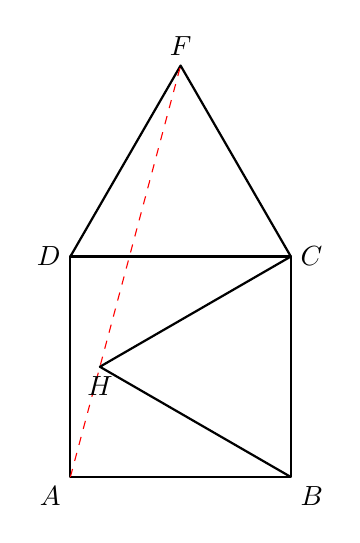
\begin{tikzpicture}[scale=0.7, line join=round]
				% Définition des points du carré (côté 4cm)
				\coordinate (A) at (0,0);
				\coordinate (B) at (4,0);
				\coordinate (C) at (4,4);
				\coordinate (D) at (0,4);

				% Tracé du carré
				\draw[thick] (A) -- (B) -- (C) -- (D) -- cycle;

				% Triangle équilatéral DFC (vers le haut)
				% La hauteur est 4 * sin(60°) = 2*sqrt(3)
				\coordinate (F) at (2,{4 + 2*sqrt(3)});
				\draw[thick] (D) -- (F) -- (C);

				% Triangle équilatéral BCH (vers l'intérieur)
				% La pointe H est à 4 - 2*sqrt(3) du bord droit
				\coordinate (H) at ({4 - 2*sqrt(3)}, 2);
				\draw[thick] (B) -- (H) -- (C);

				% Tracé de la ligne pour démontrer l'alignement (A, H, F)
				\draw[dashed, red] (A) -- (F);

				% Étiquettes des points
				\node[below left] at (A) {$A$};
				\node[below right] at (B) {$B$};
				\node[right] at (C) {$C$};
				\node[left] at (D) {$D$};
				\node[above] at (F) {$F$};
				\node[below] at (H) {$H$};
			\end{tikzpicture}
		\end{center}
	\end{exo}

	\begin{exo}{}
		\begin{center}
			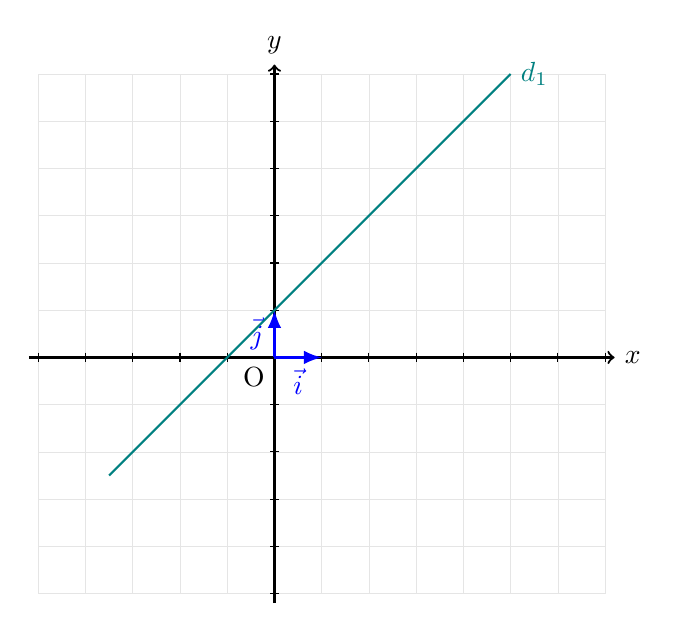
\begin{tikzpicture}[scale=0.6]
				% Grille fine

				\draw[step=1, gray!20, very thin] (-5,-5) grid (7,6);
				% Axes
				\draw[thick, ->] (-5.2,0) -- (7.2,0) node[right] {$x$};
				\draw[thick, ->] (0,-5.2) -- (0,6.2) node[above] {$y$};

				% Graduation
				\foreach \x in {-5,-4,...,7}
				\draw (\x, 0.1) -- (\x, -0.1);
				\foreach \y in {-5,-4,...,6}
				\draw (0.1, \y) -- (-0.1, \y);

				% Vecteurs unitaires i et j
				\draw[very thick, -latex, blue] (0,0) -- (1,0) node[midway, below] {$\vec{i}$};
				\draw[very thick, -latex, blue] (0,0) -- (0,1) node[midway, left] {$\vec{j}$};
				\node[below left] at (0,0) {O};

				% Exemple : Tracé de la droite d1 (exercice 37)
				% Si on prend une droite passant par (-1,0) et (1,2)
				\draw[domain=-3.5:5, thick, teal] plot (\x, {\x + 1}) node[right] {$d_1$};
			\end{tikzpicture}
		\end{center}
	\end{exo}

\end{multicols}

\end{document}
